\subsubsection{MF4. Módulo de interfaz de usuario}

\paragraph{MF4.1}


\begin{figure}[!htb]
    \centering
    \begin{subfigure}{0.45\textwidth}
        \centering
        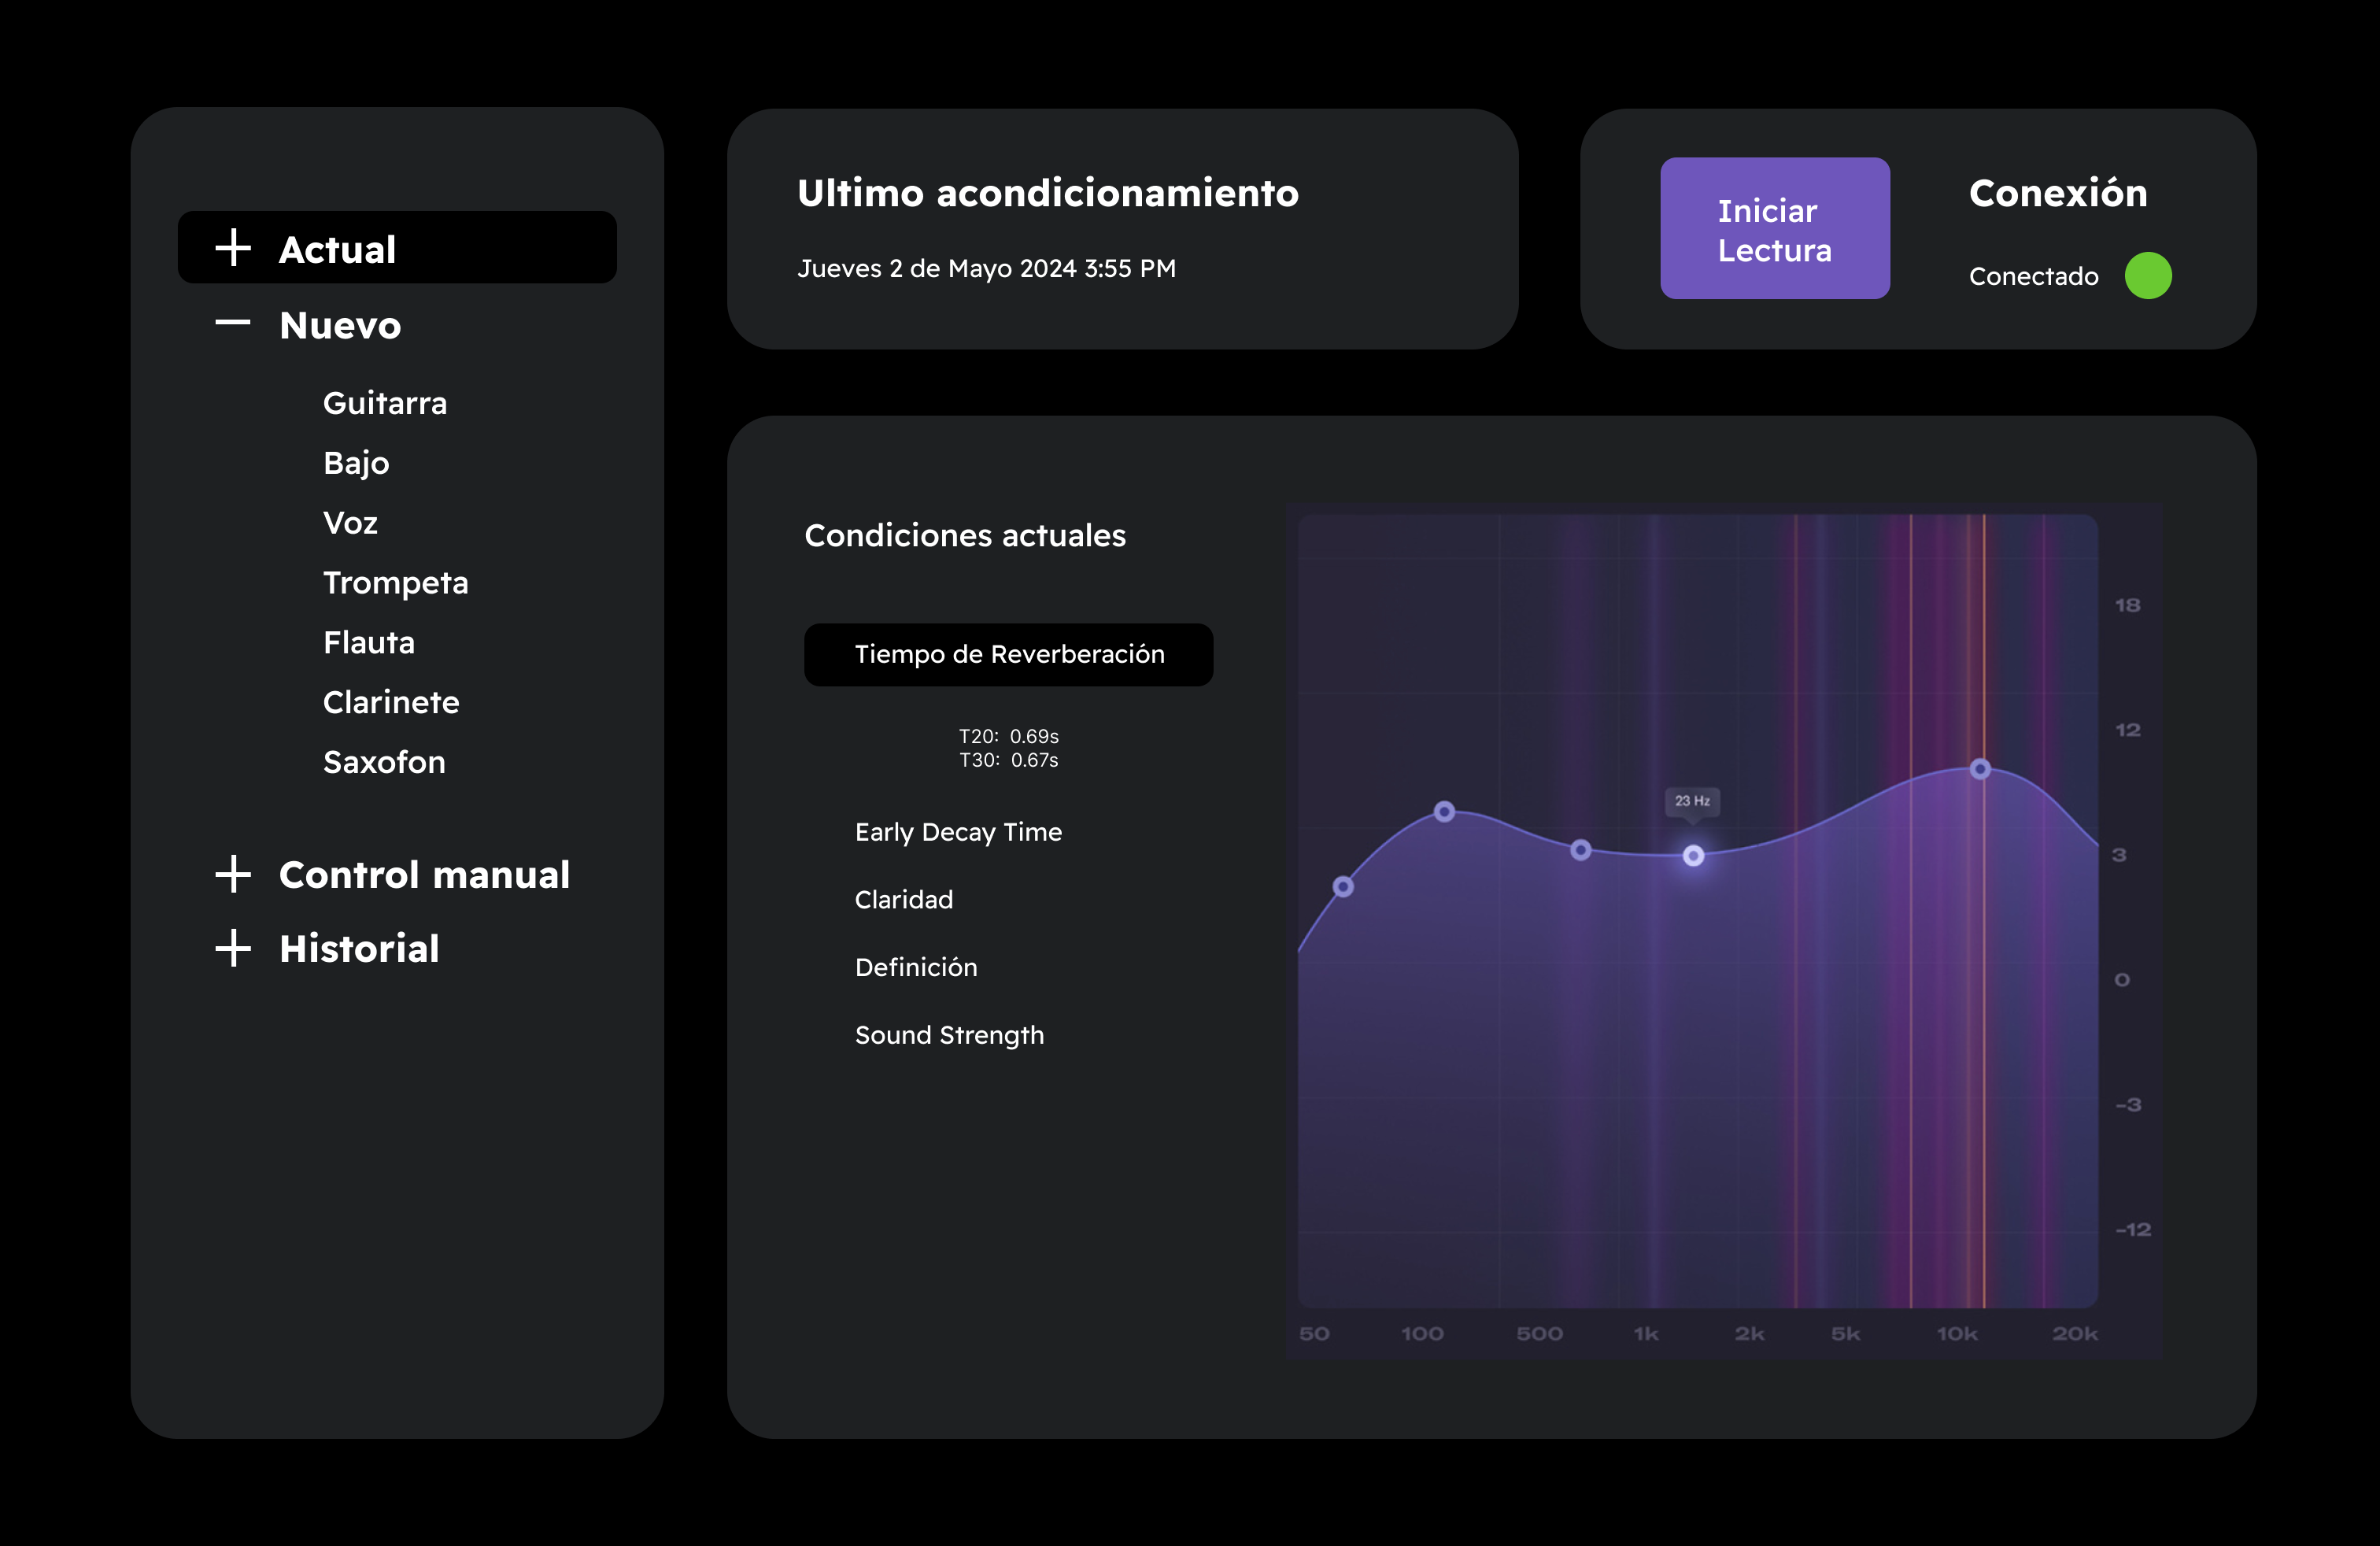
\includegraphics[width=\linewidth]{imagenes/Landing.png}
        \caption{\footnotesize Señal de excitación (Barrido senoidal)}
        \label{fig:sub1}
    \end{subfigure}
    \hfill
    \begin{subfigure}{0.45\textwidth}
        \centering
        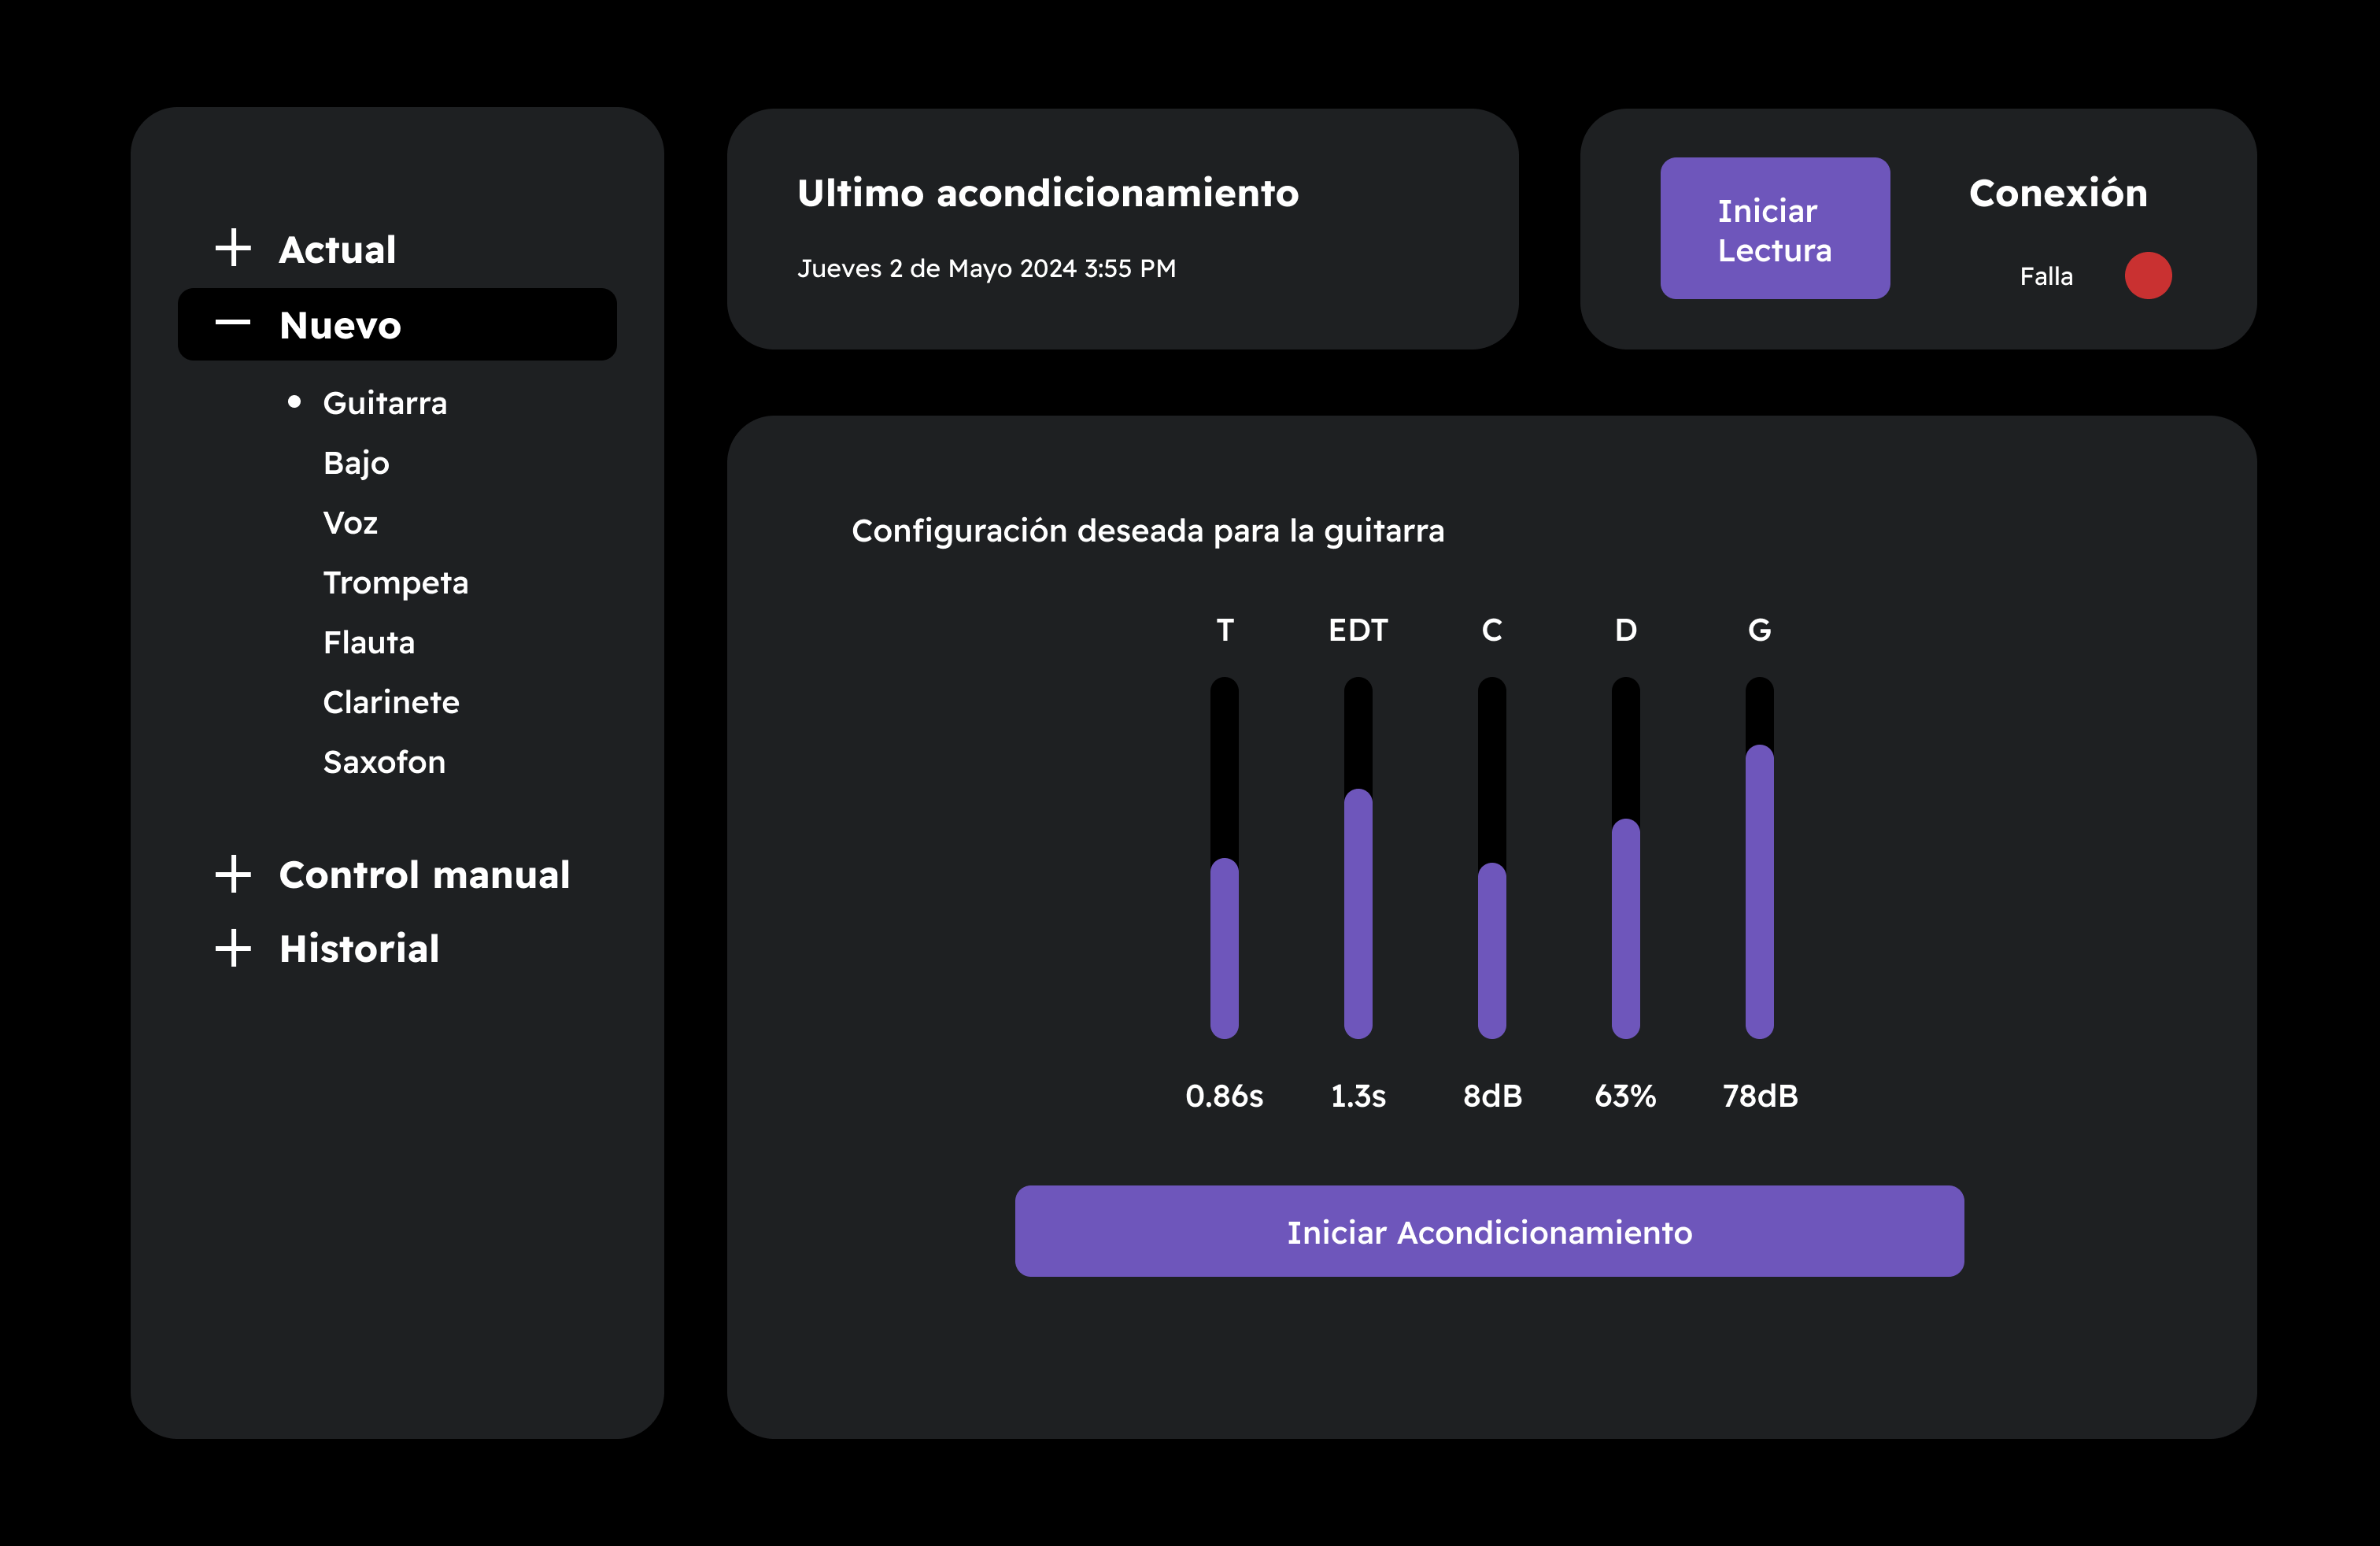
\includegraphics[width=\linewidth]{imagenes/Guitarra.png}
        \caption{\footnotesize Audio grabado}
        \label{fig:sub2}
    \end{subfigure}
    \vskip\baselineskip
    \begin{subfigure}{0.45\textwidth}
        \centering
        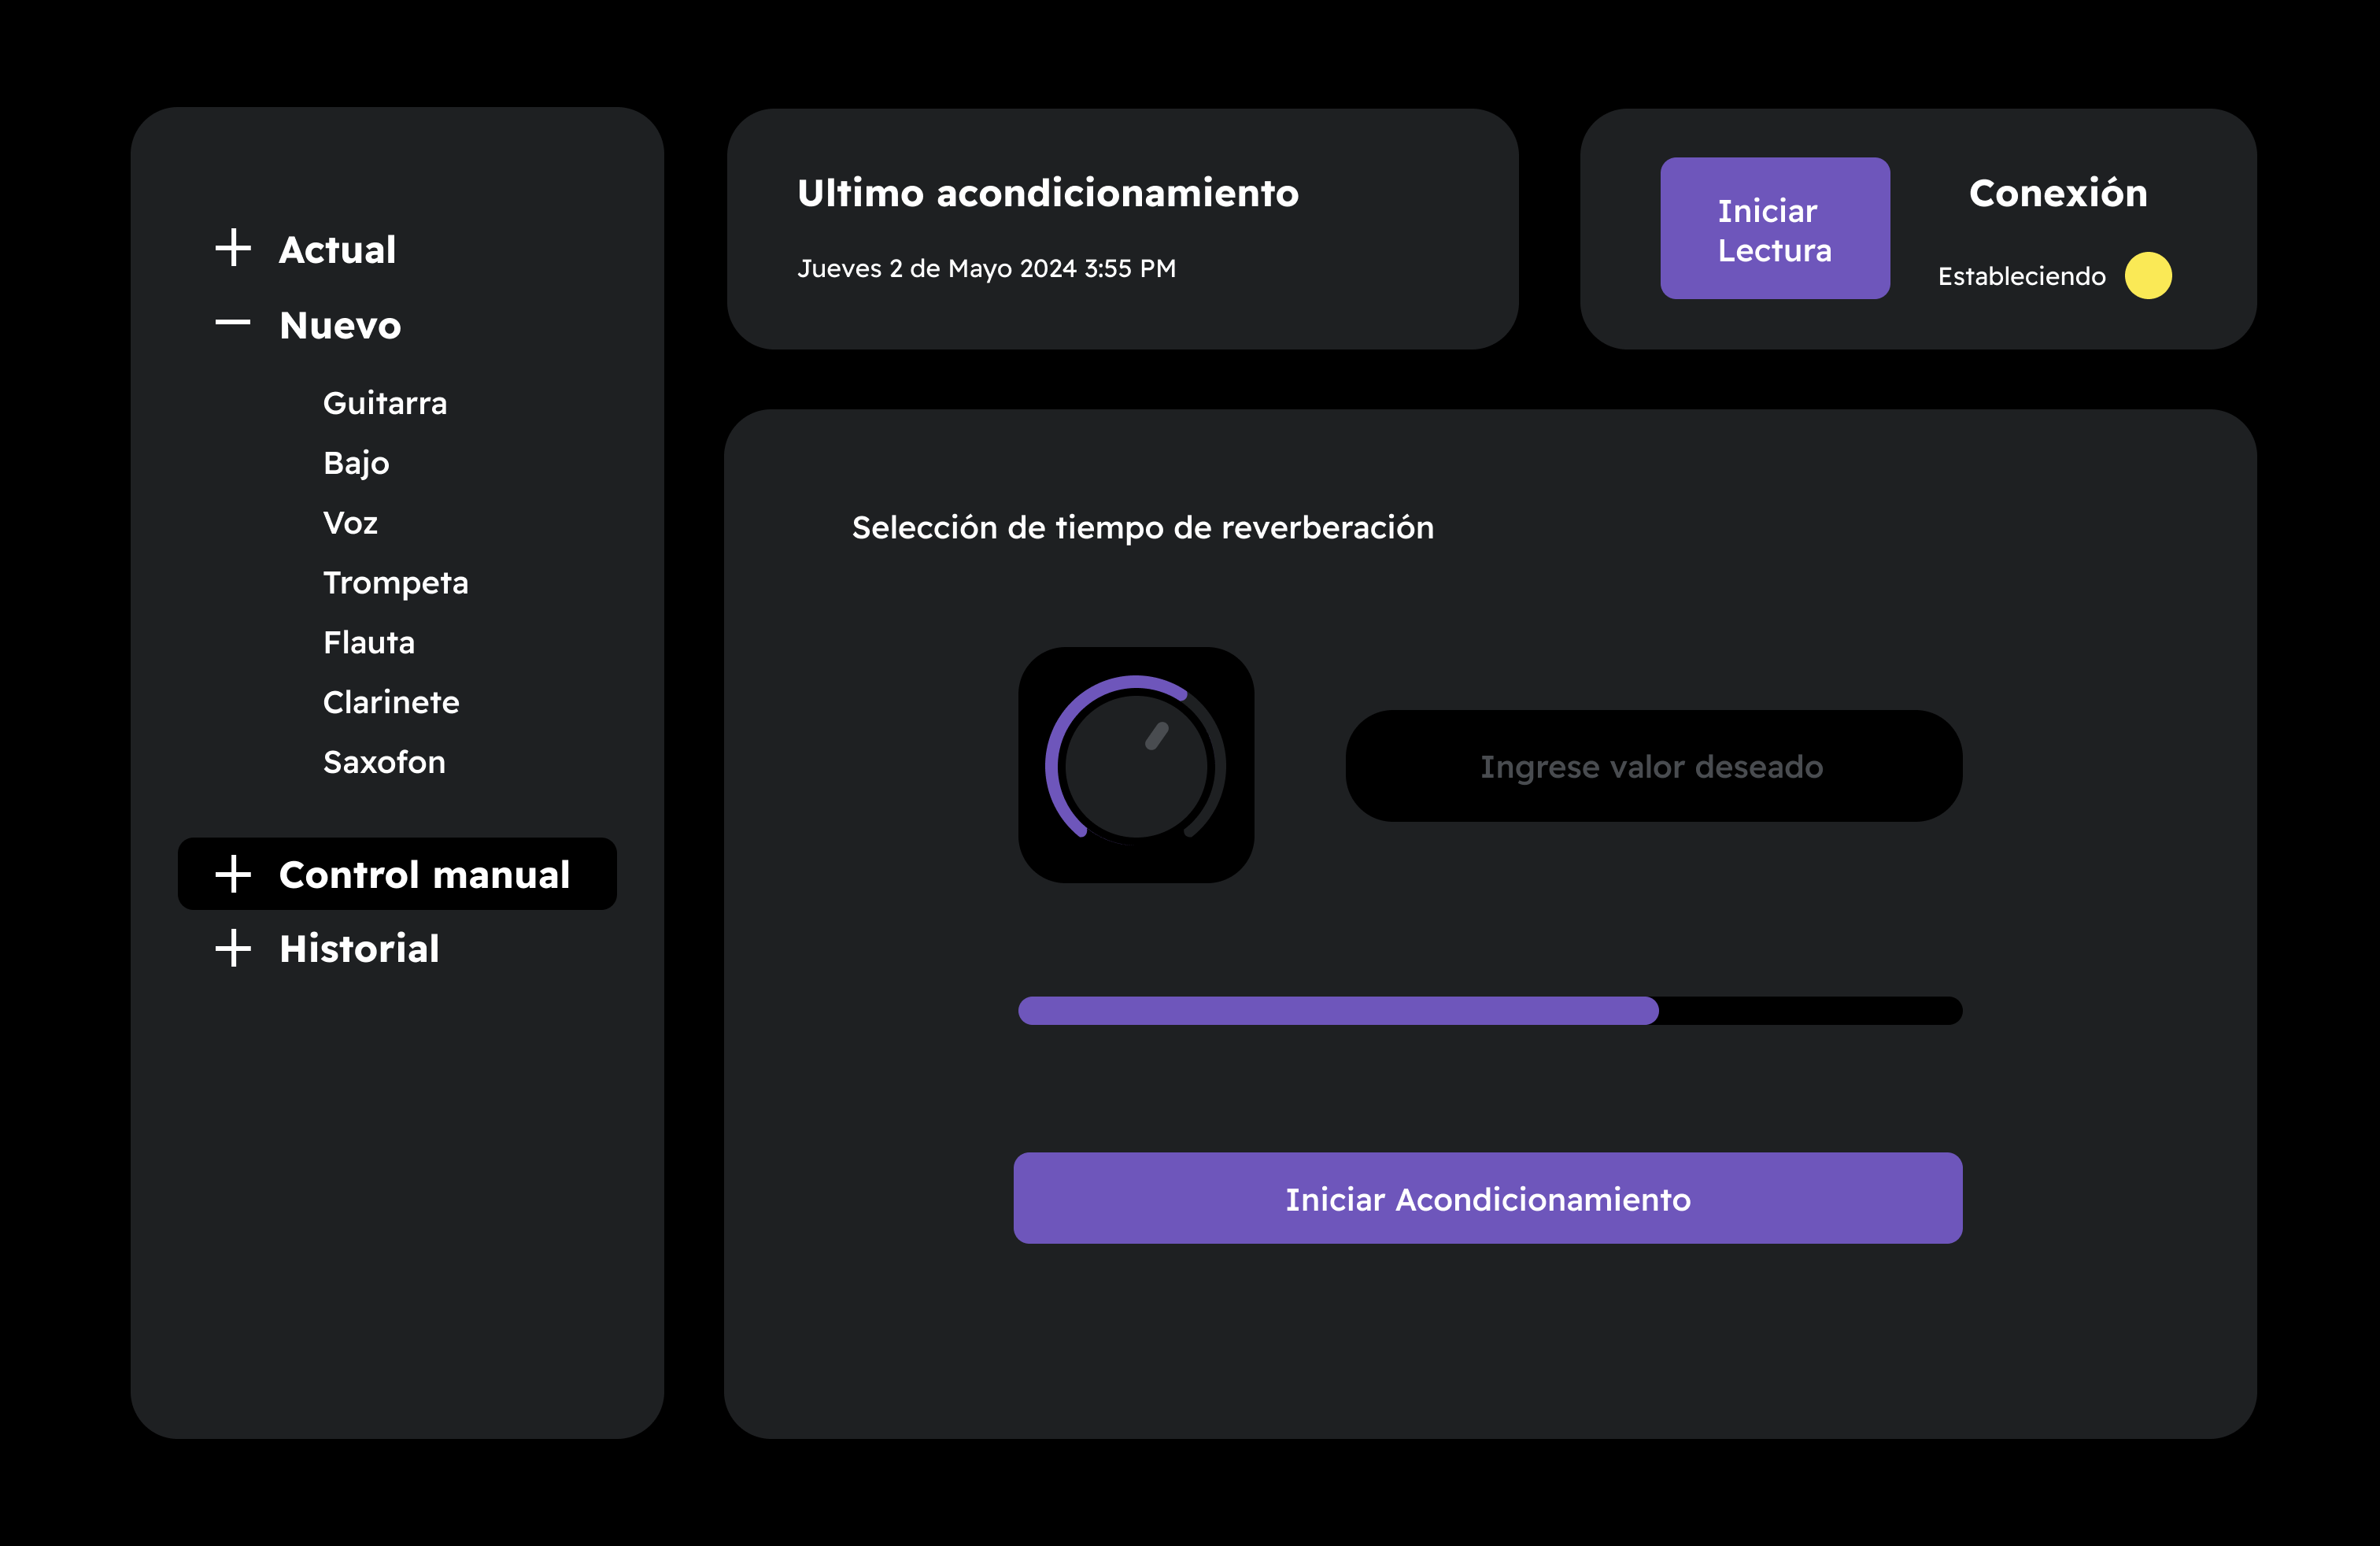
\includegraphics[width=\linewidth]{imagenes/Control Manual.png}
        \caption{\footnotesize Respuesta al impulso estimada}
        \label{fig:sub3}
    \end{subfigure}
    \hfill
    \begin{subfigure}{0.45\textwidth}
        \centering
        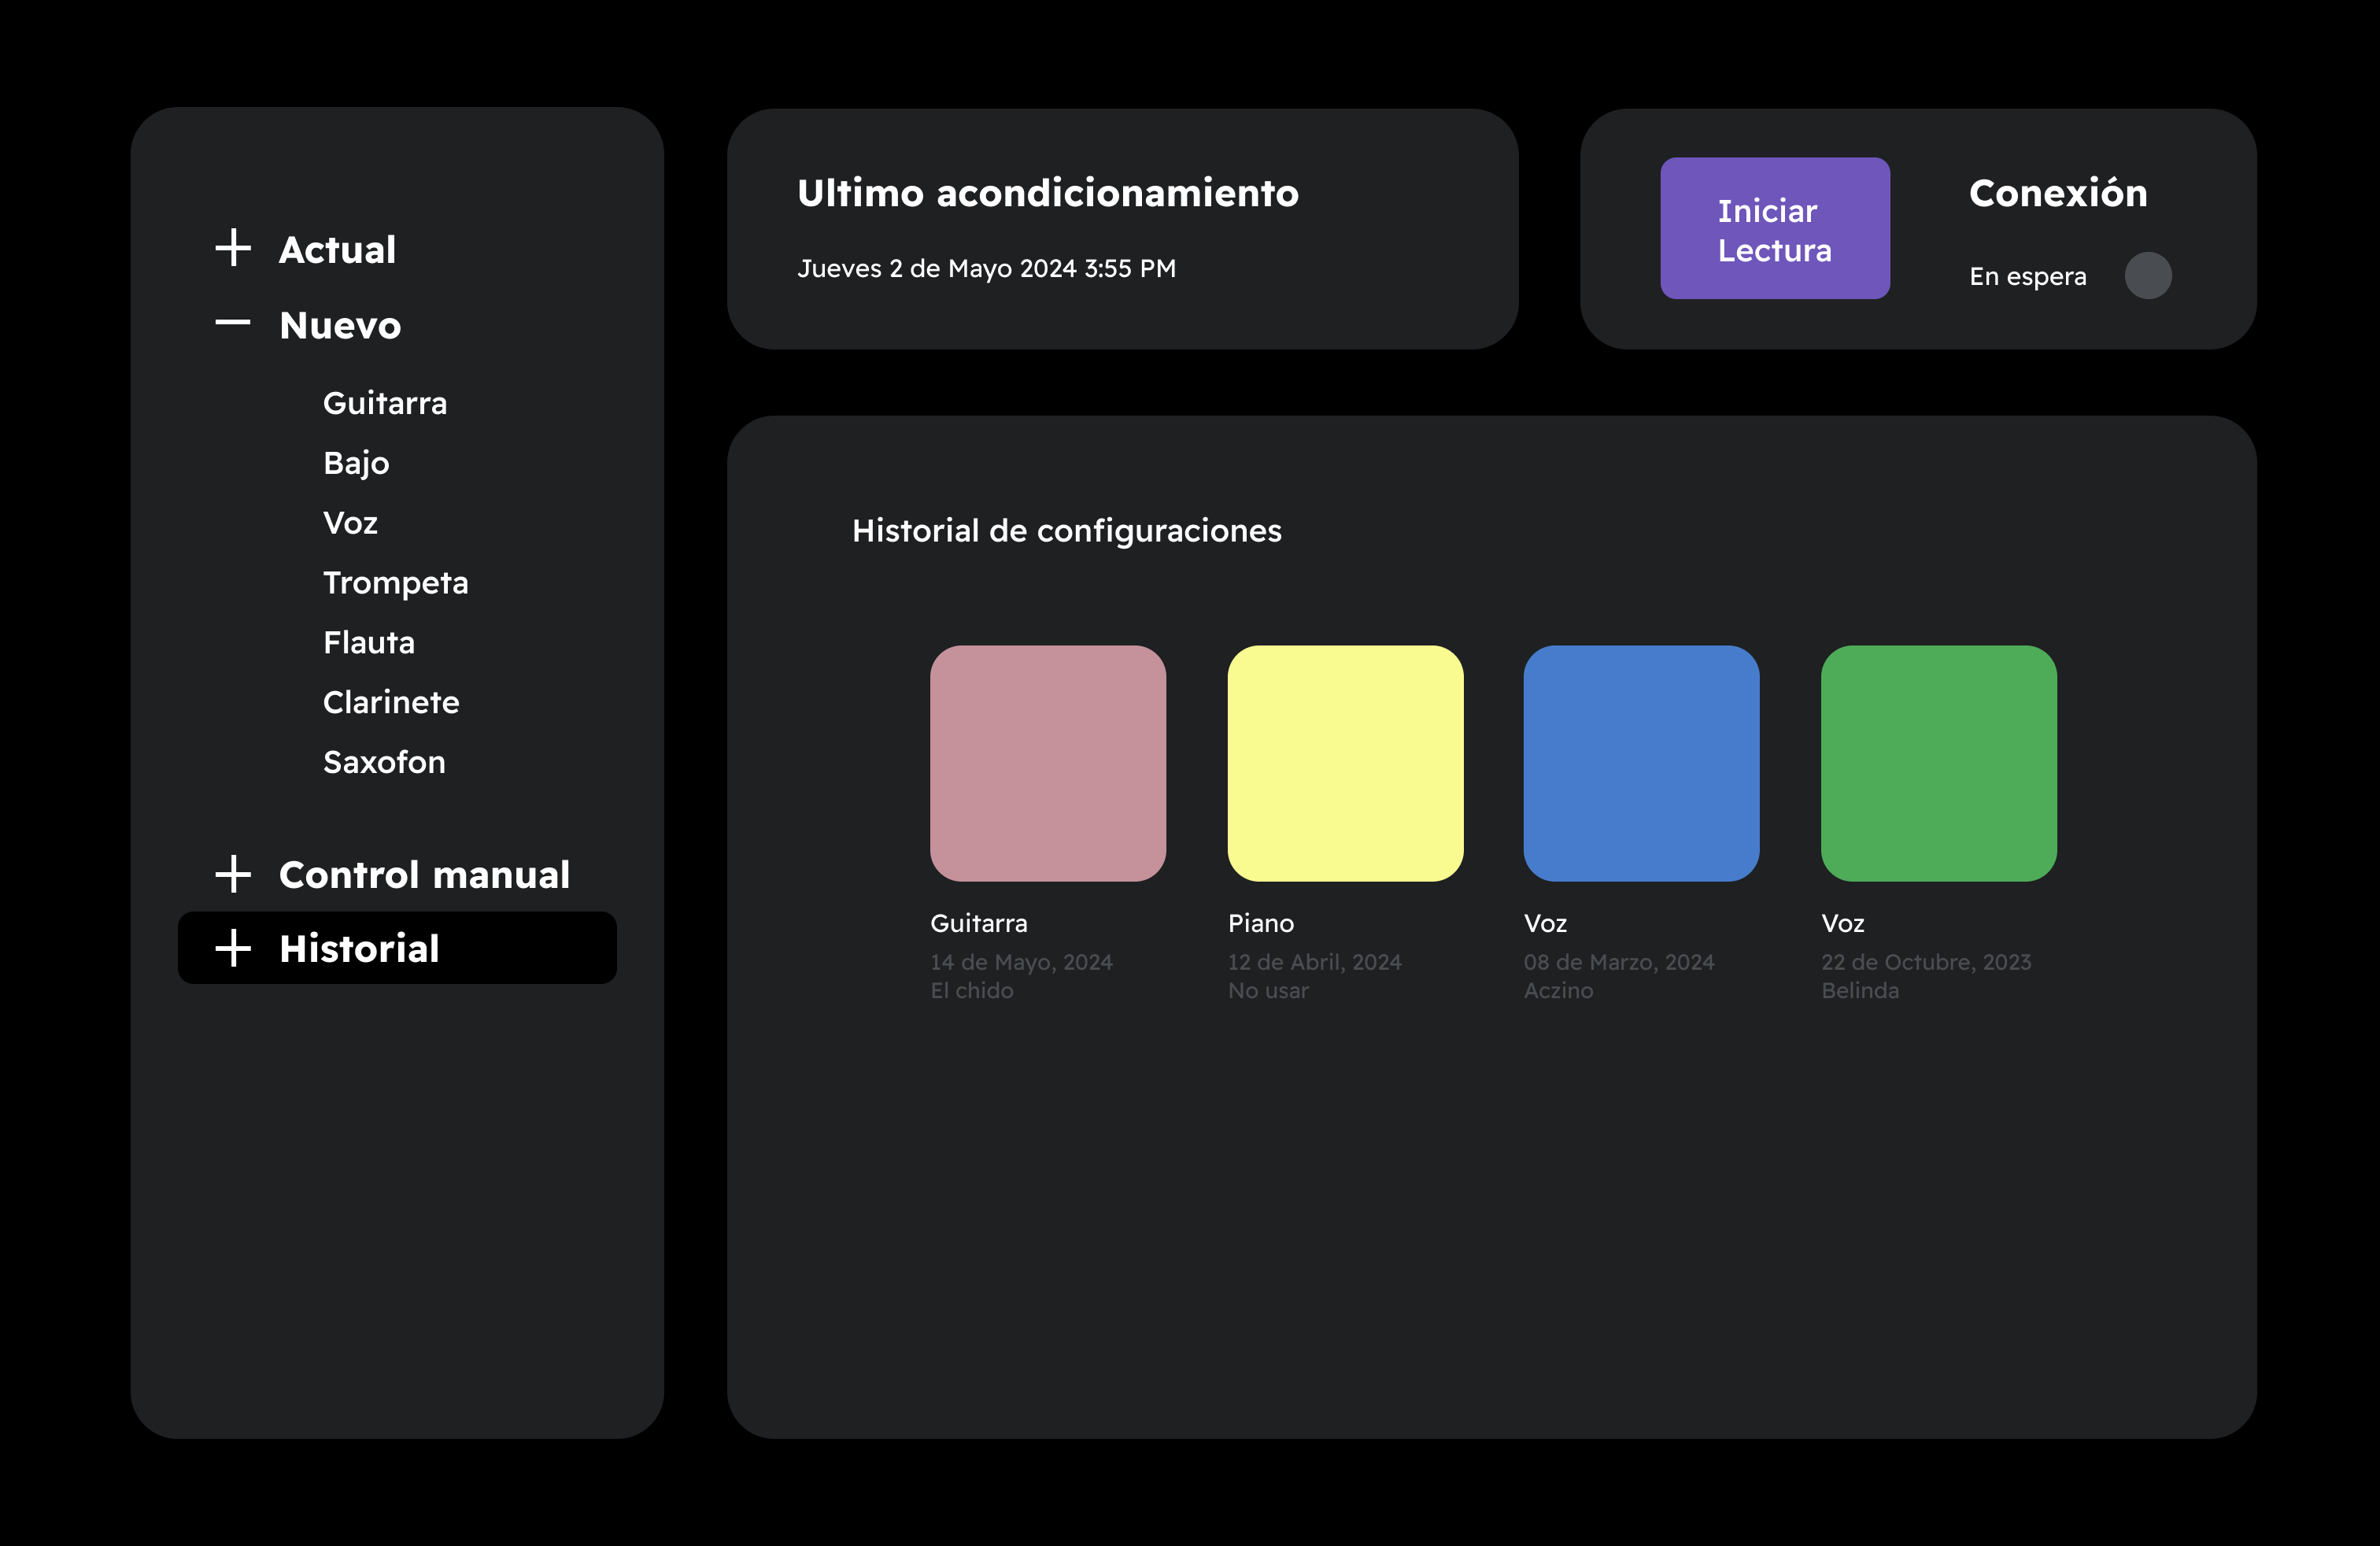
\includegraphics[width=\linewidth]{imagenes/Historial.png}
        \caption{\footnotesize Audio grabado}
        \label{fig:sub4}
    \end{subfigure}
    \caption{Gráficas resultantes de generación y medición de la acústica}
\end{figure}

\hfill\break
\begin{figure}[!htb]
    \centering
    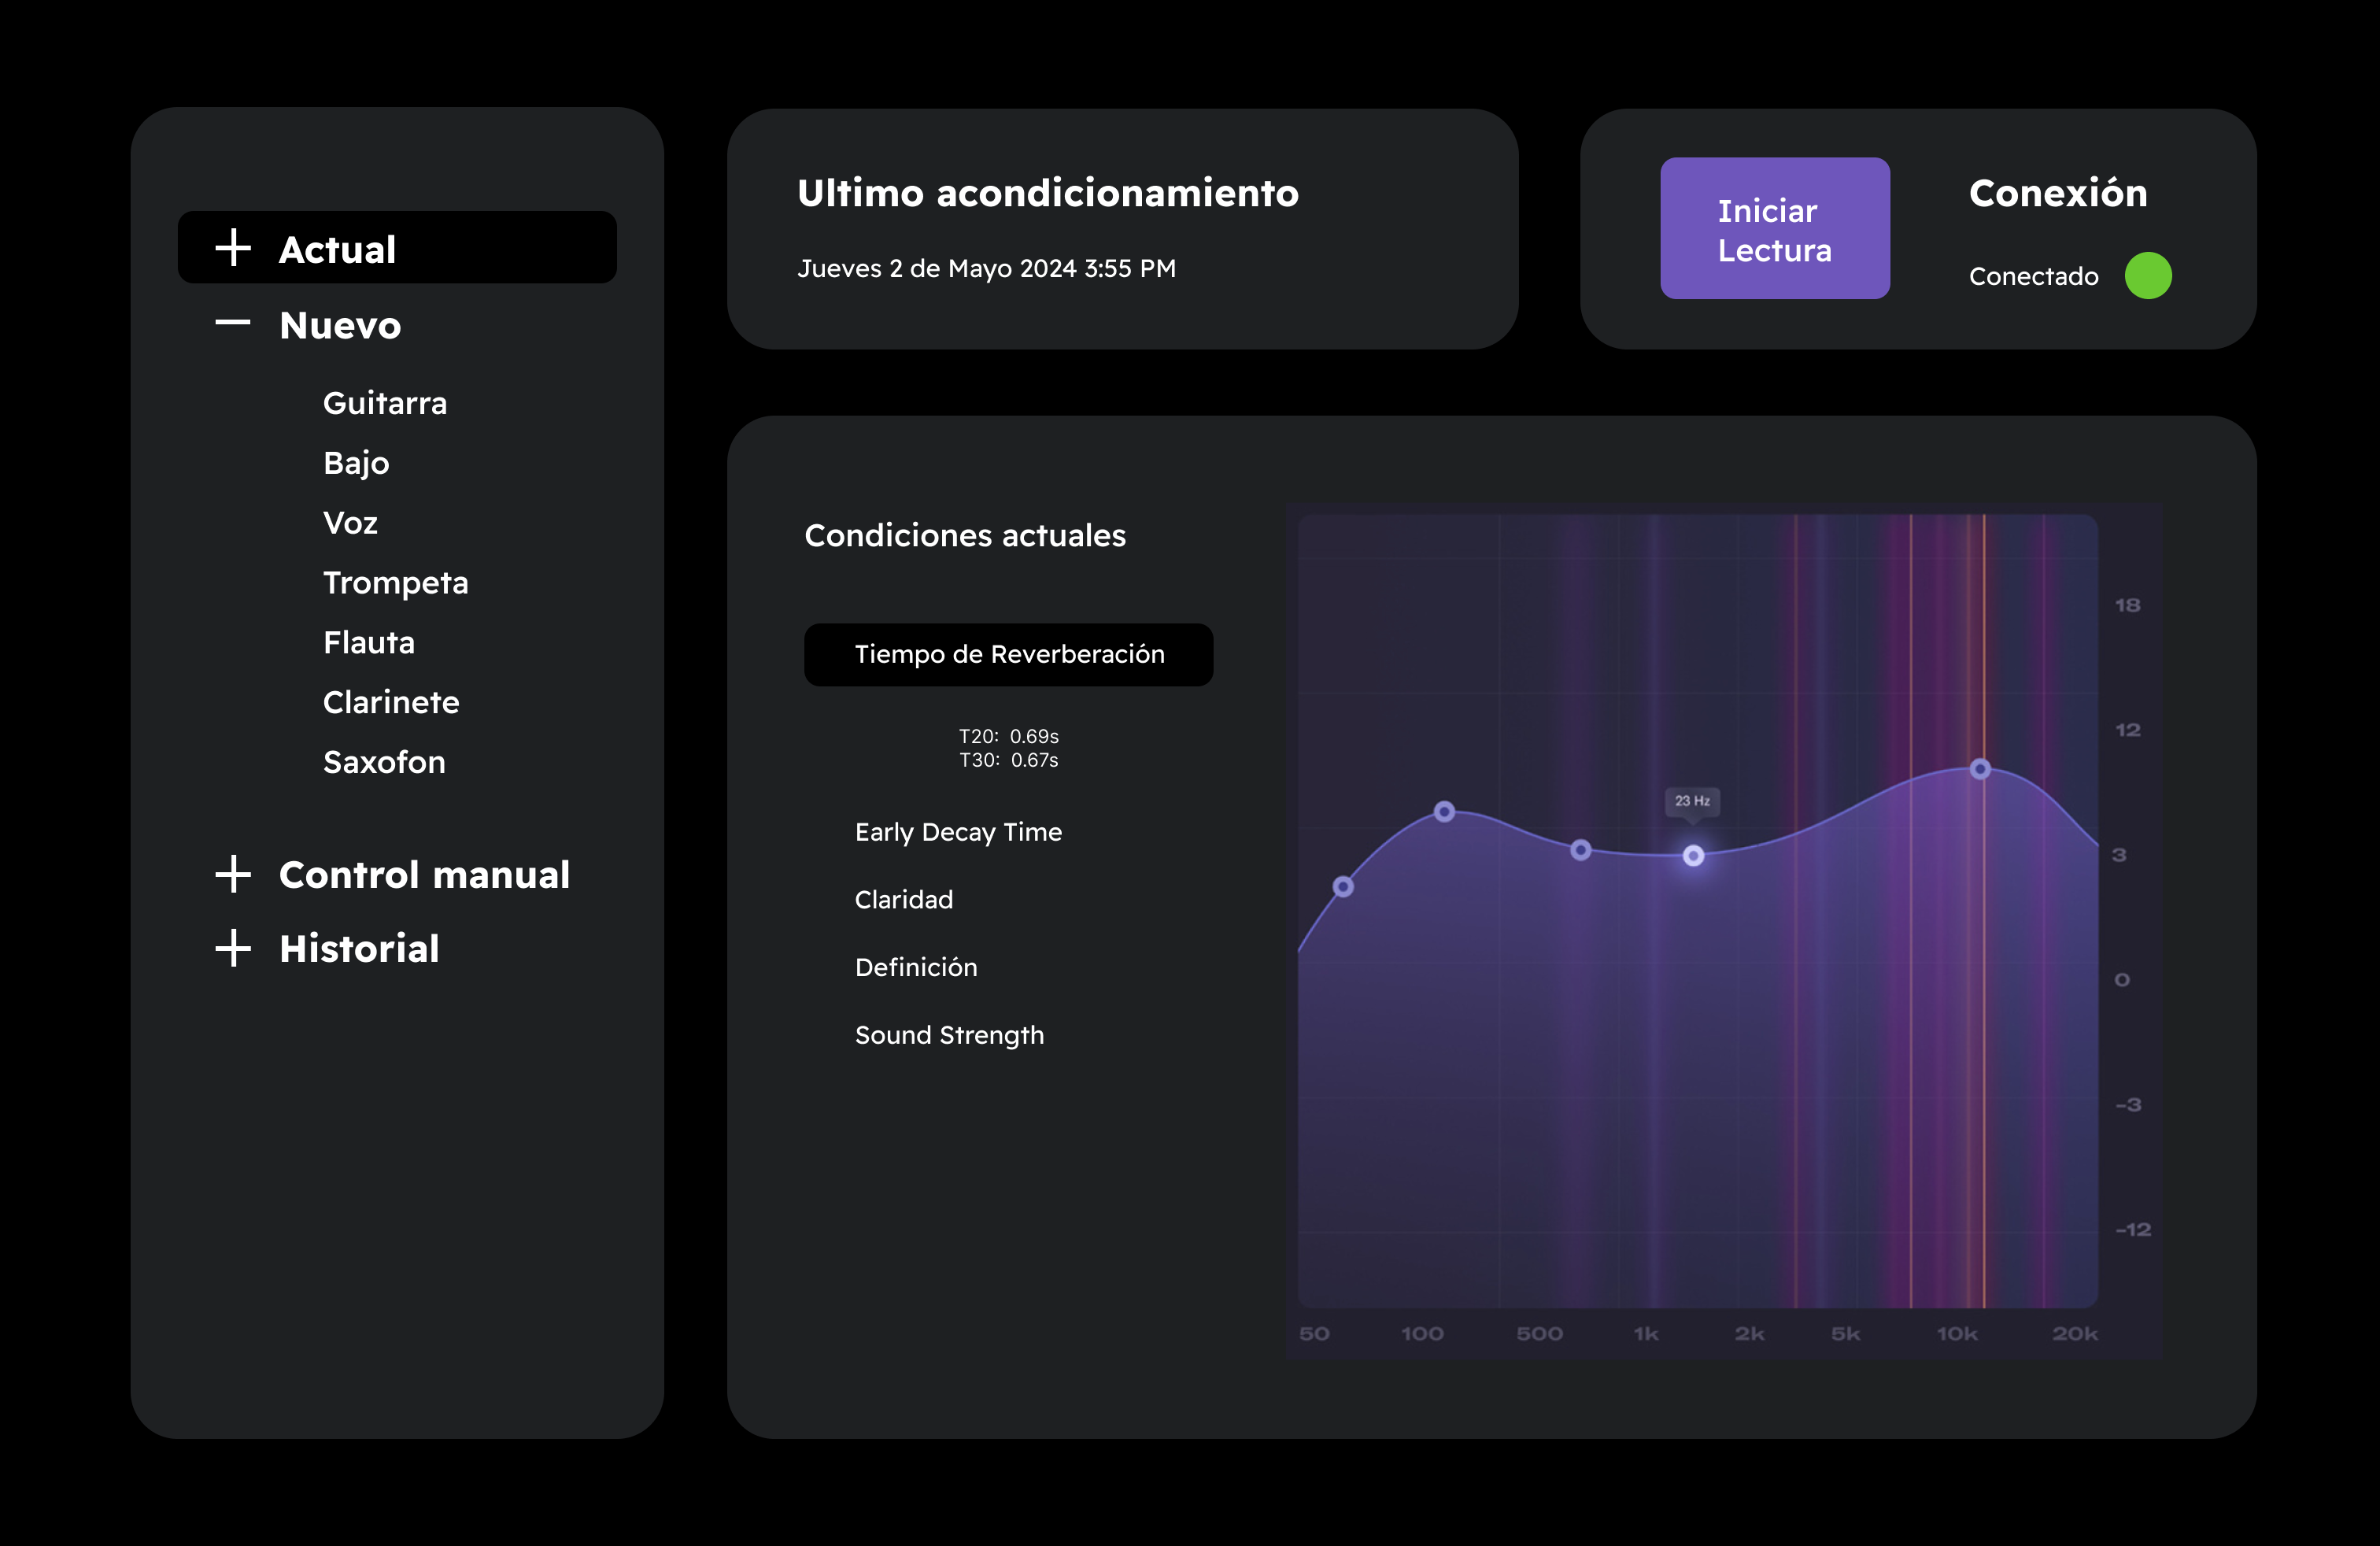
\includegraphics[width=0.8\linewidth]{imagenes/Landing.png}
    \caption{\footnotesize Interfaz de usuario. Página de la acústica actual}
    \label{fig:DecayCurve}
\end{figure}
\FloatBarrier

\hfill\break
\begin{figure}[!htb]
    \centering
    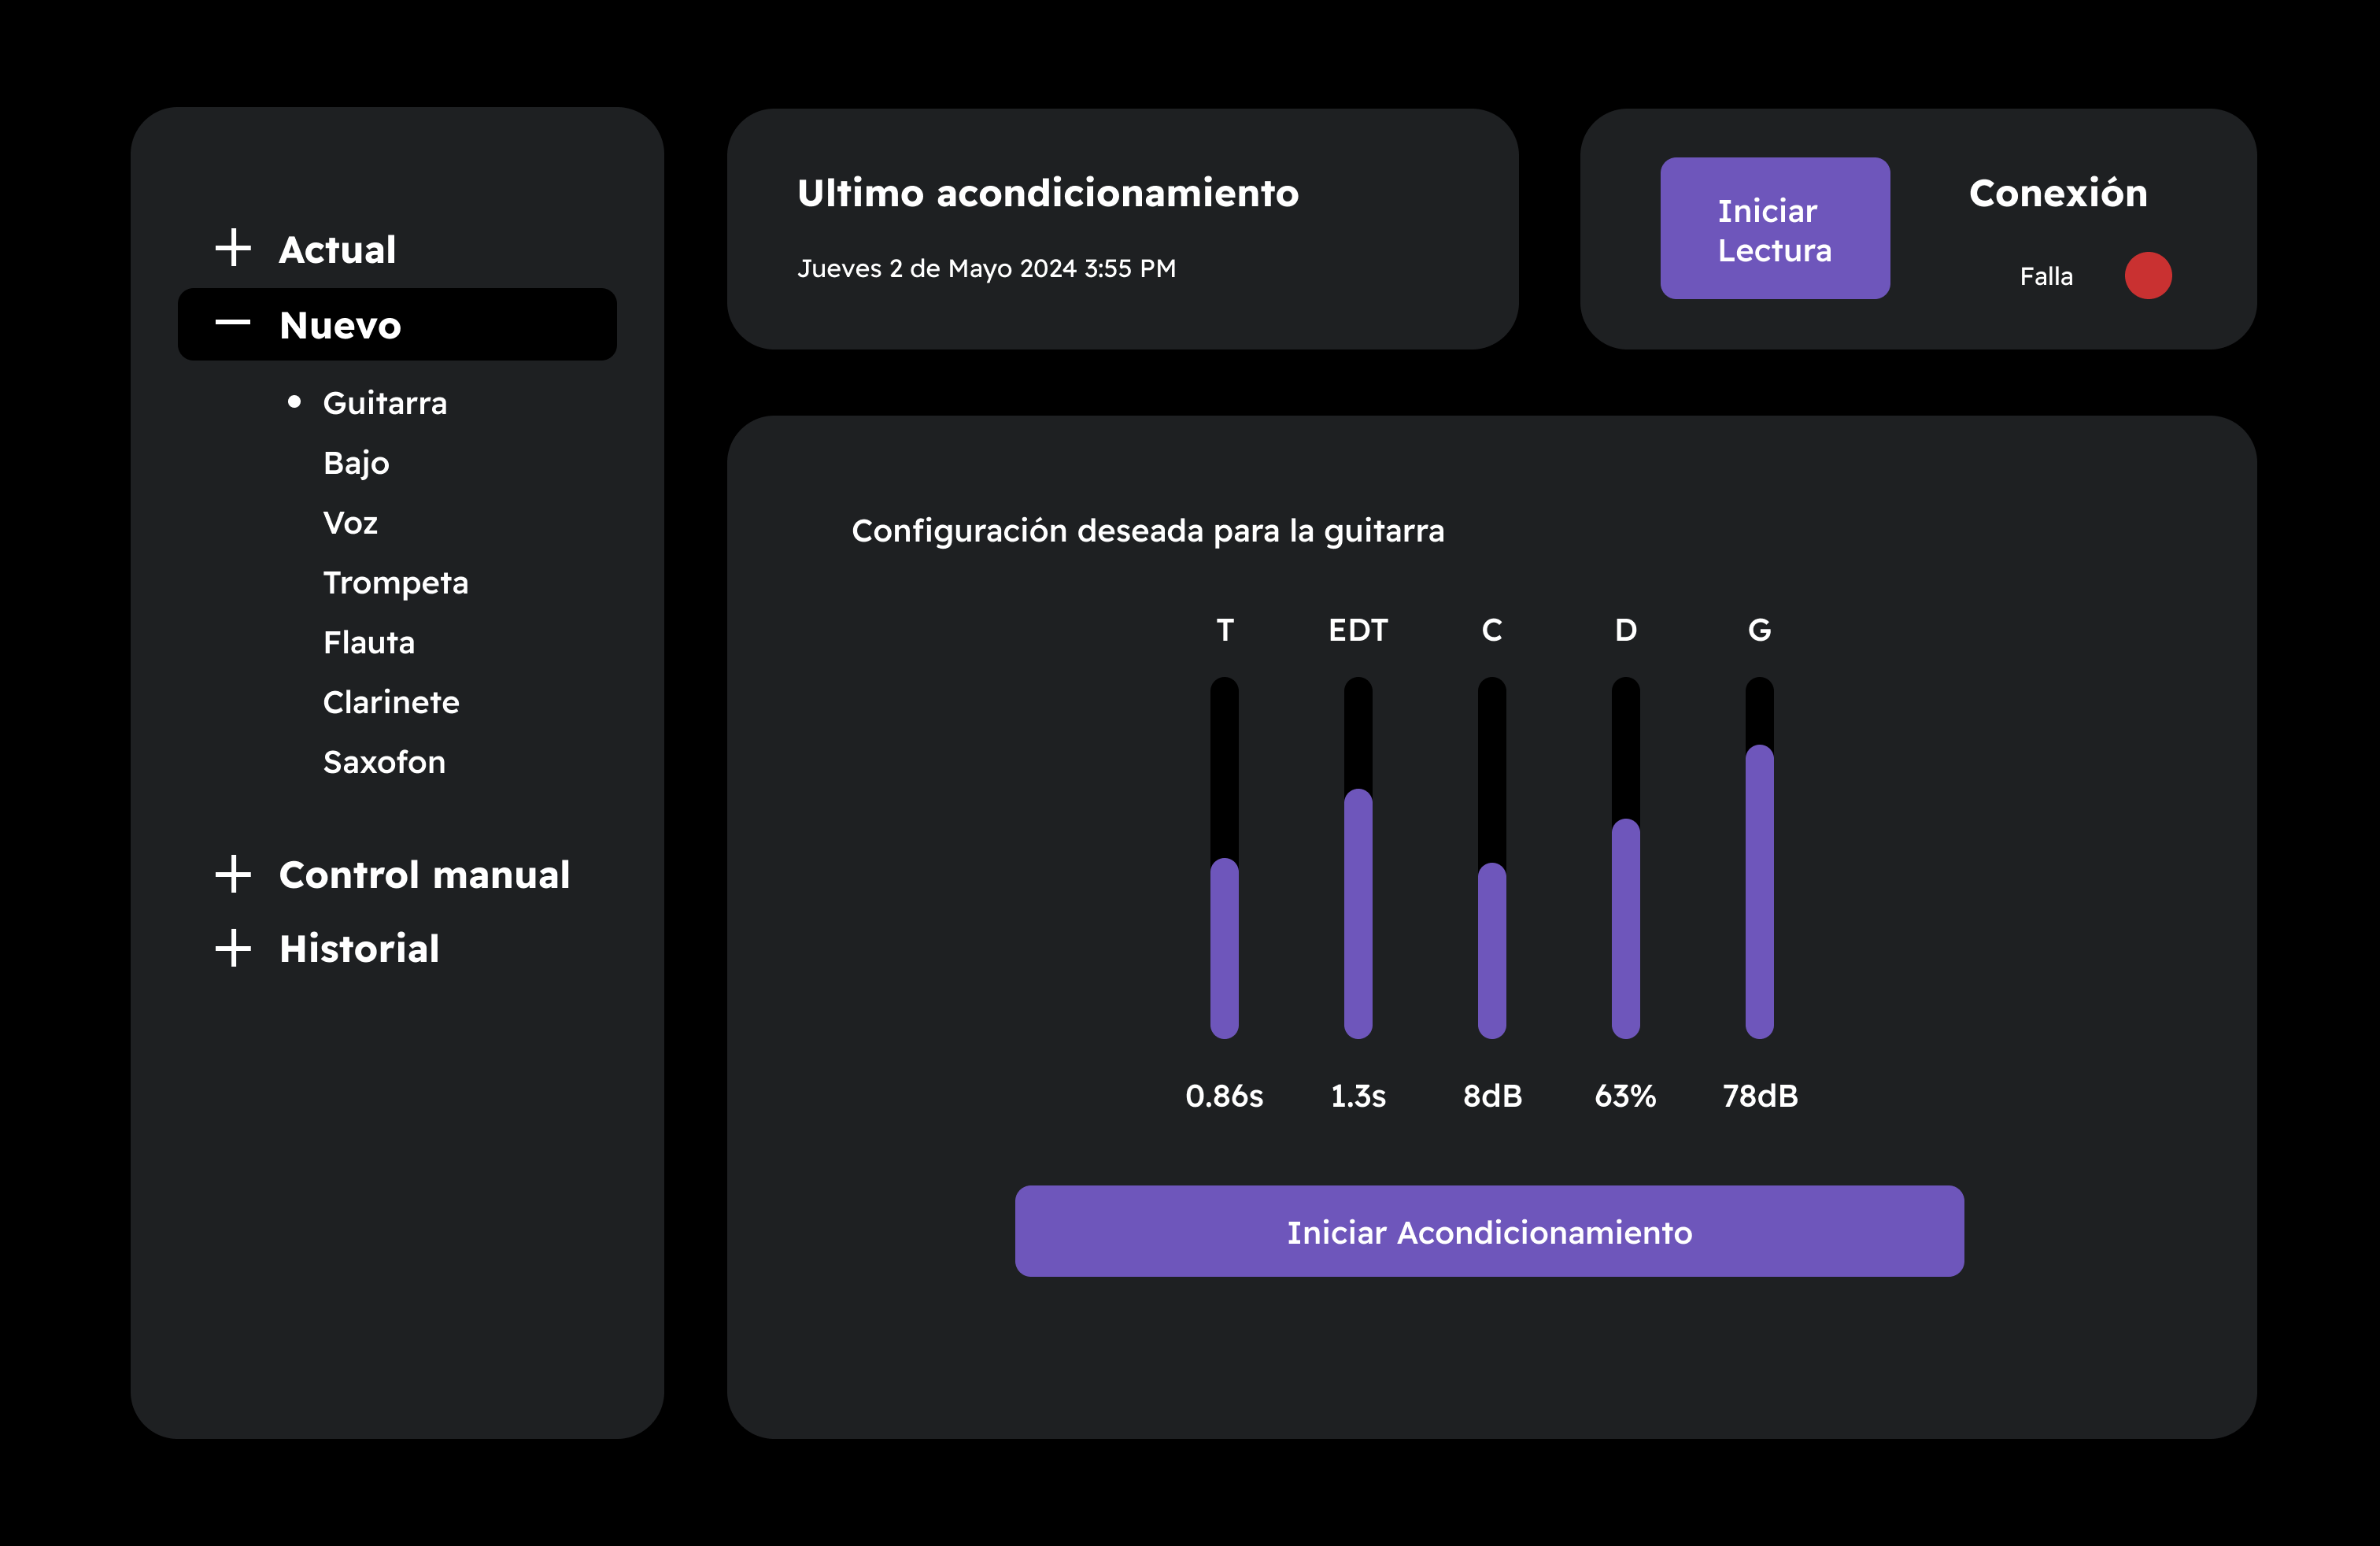
\includegraphics[width=0.8\linewidth]{imagenes/Guitarra.png}
    \caption{\footnotesize Interfaz de usuario. Página generación de una nueva acústica}
    \label{fig:DecayCurve}
\end{figure}
\FloatBarrier

\hfill\break
\begin{figure}[!htb]
    \centering
    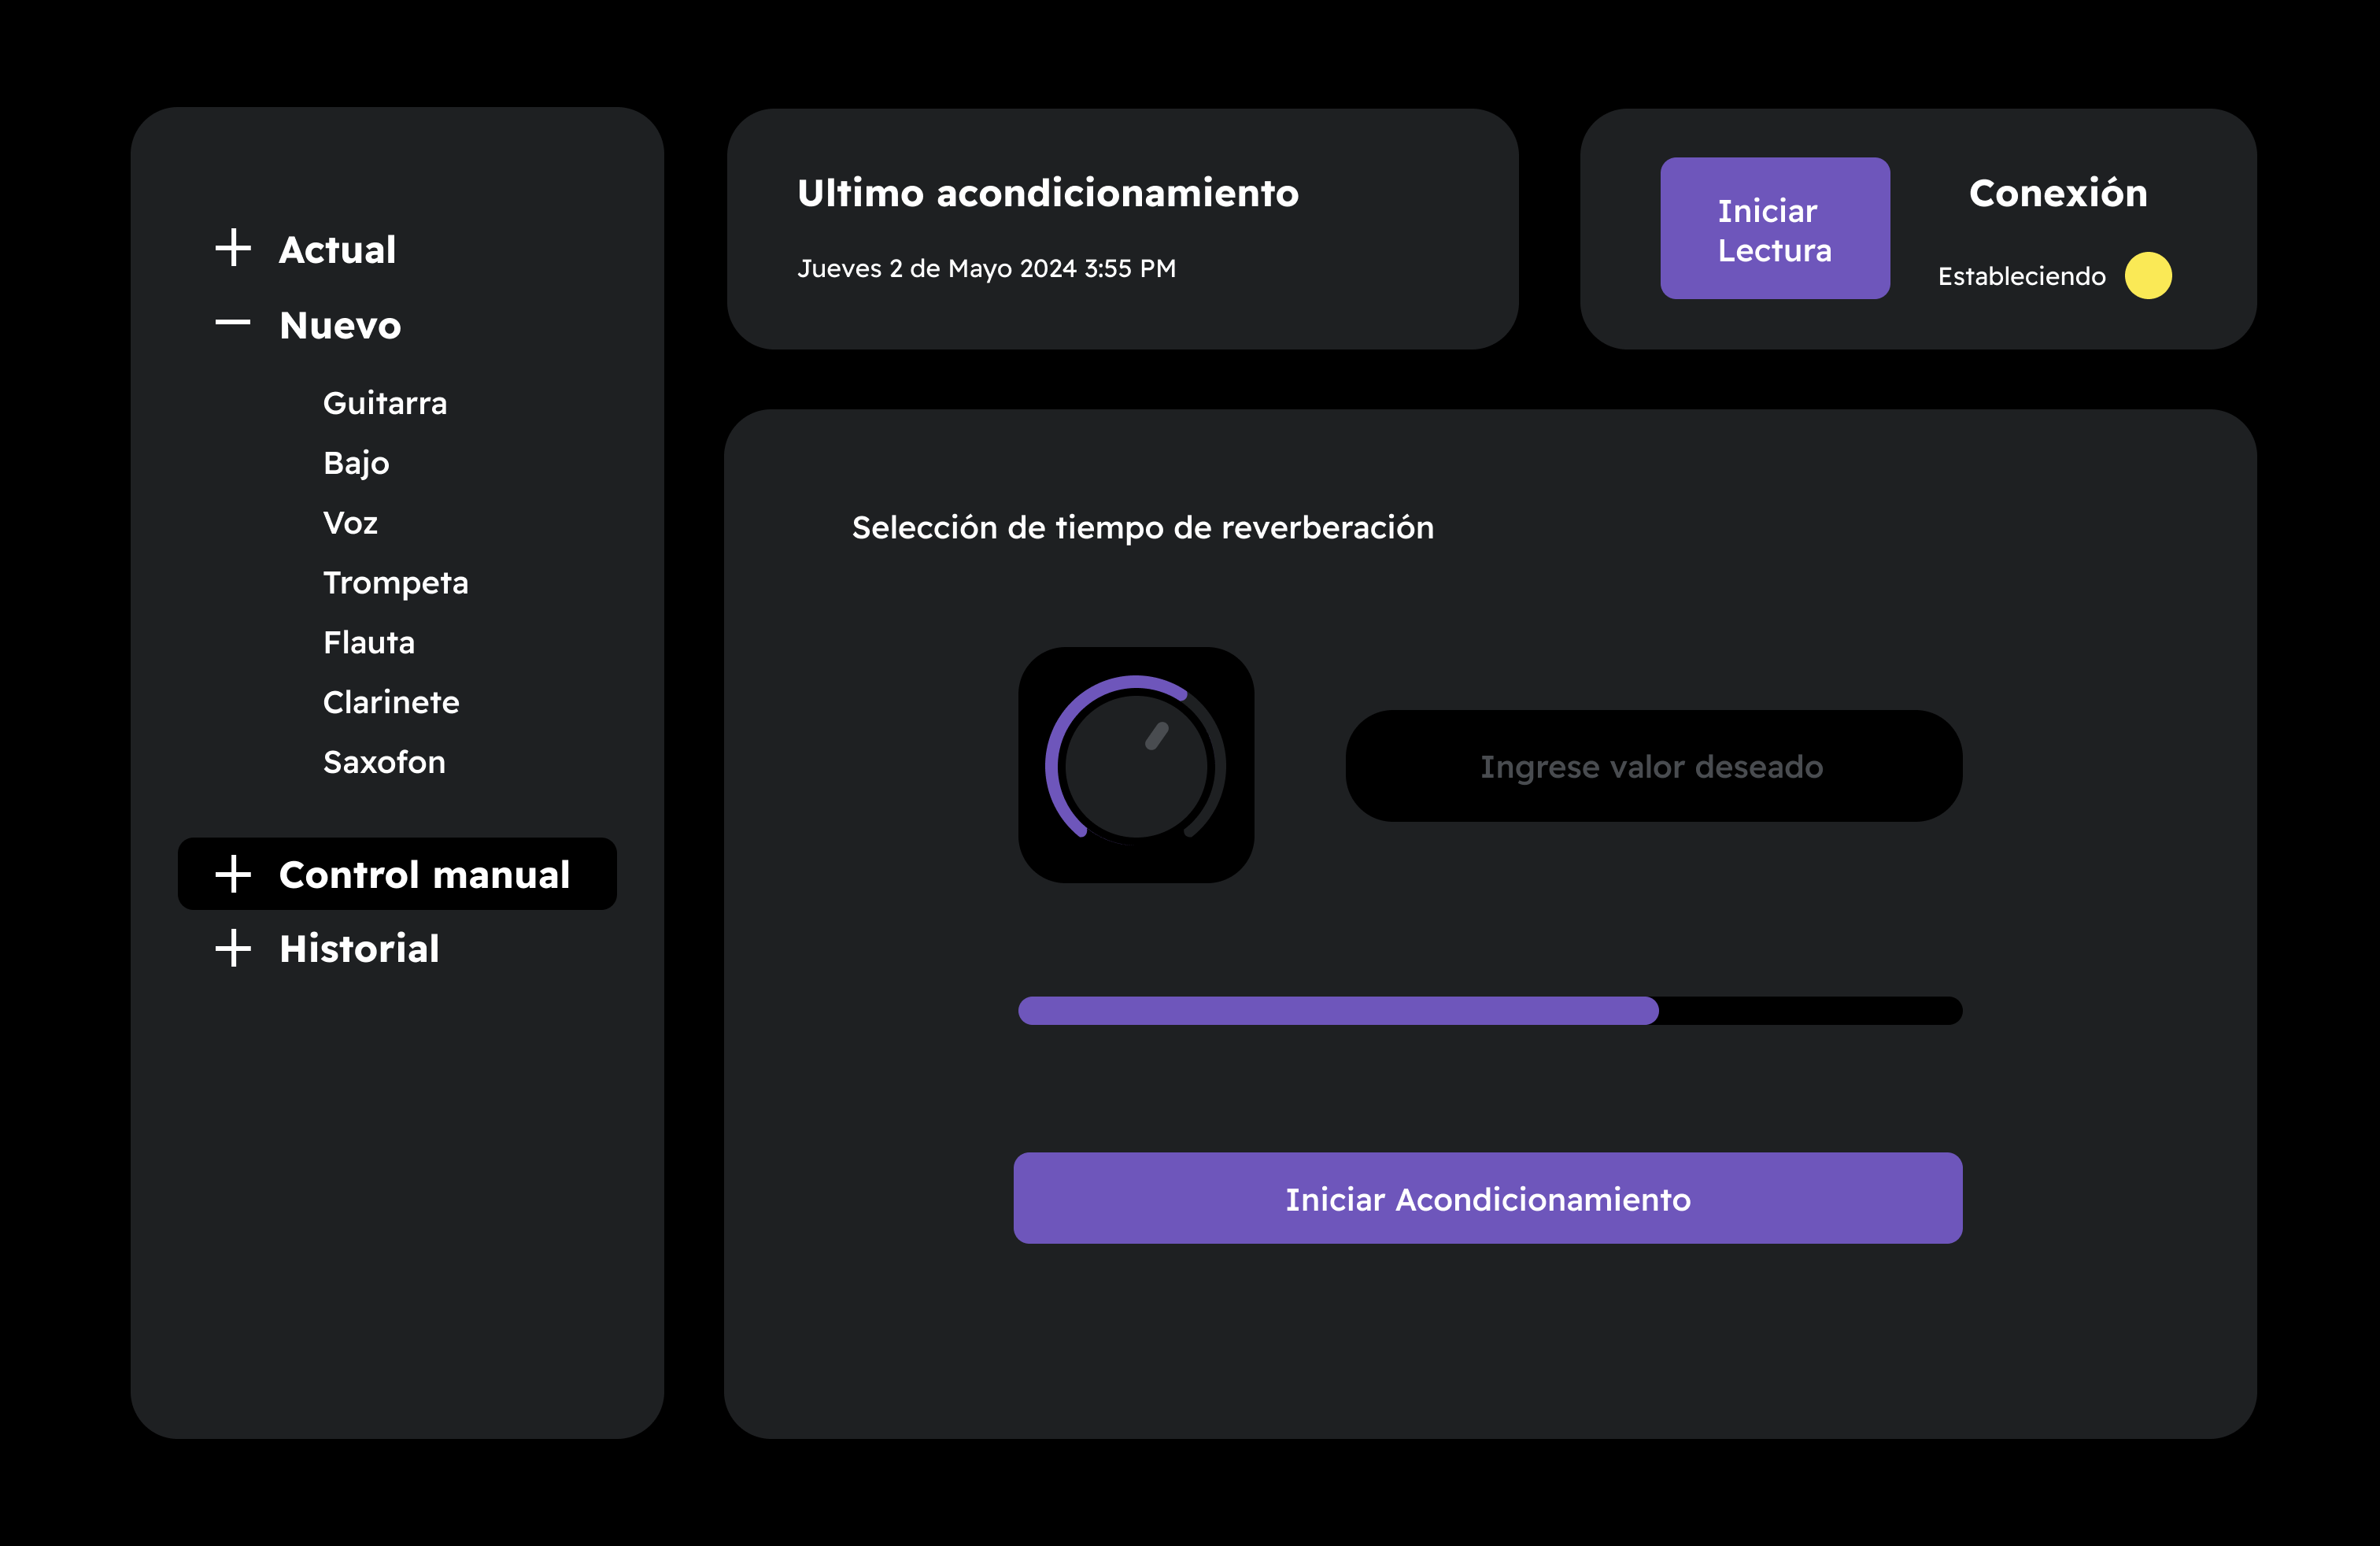
\includegraphics[width=\linewidth]{imagenes/Control Manual.png}
    \caption{\footnotesize Interfaz de usuario. Página de control manual}
    \label{fig:DecayCurve}
\end{figure}
\FloatBarrier

\hfill\break
\begin{figure}[!htb]
    \centering
    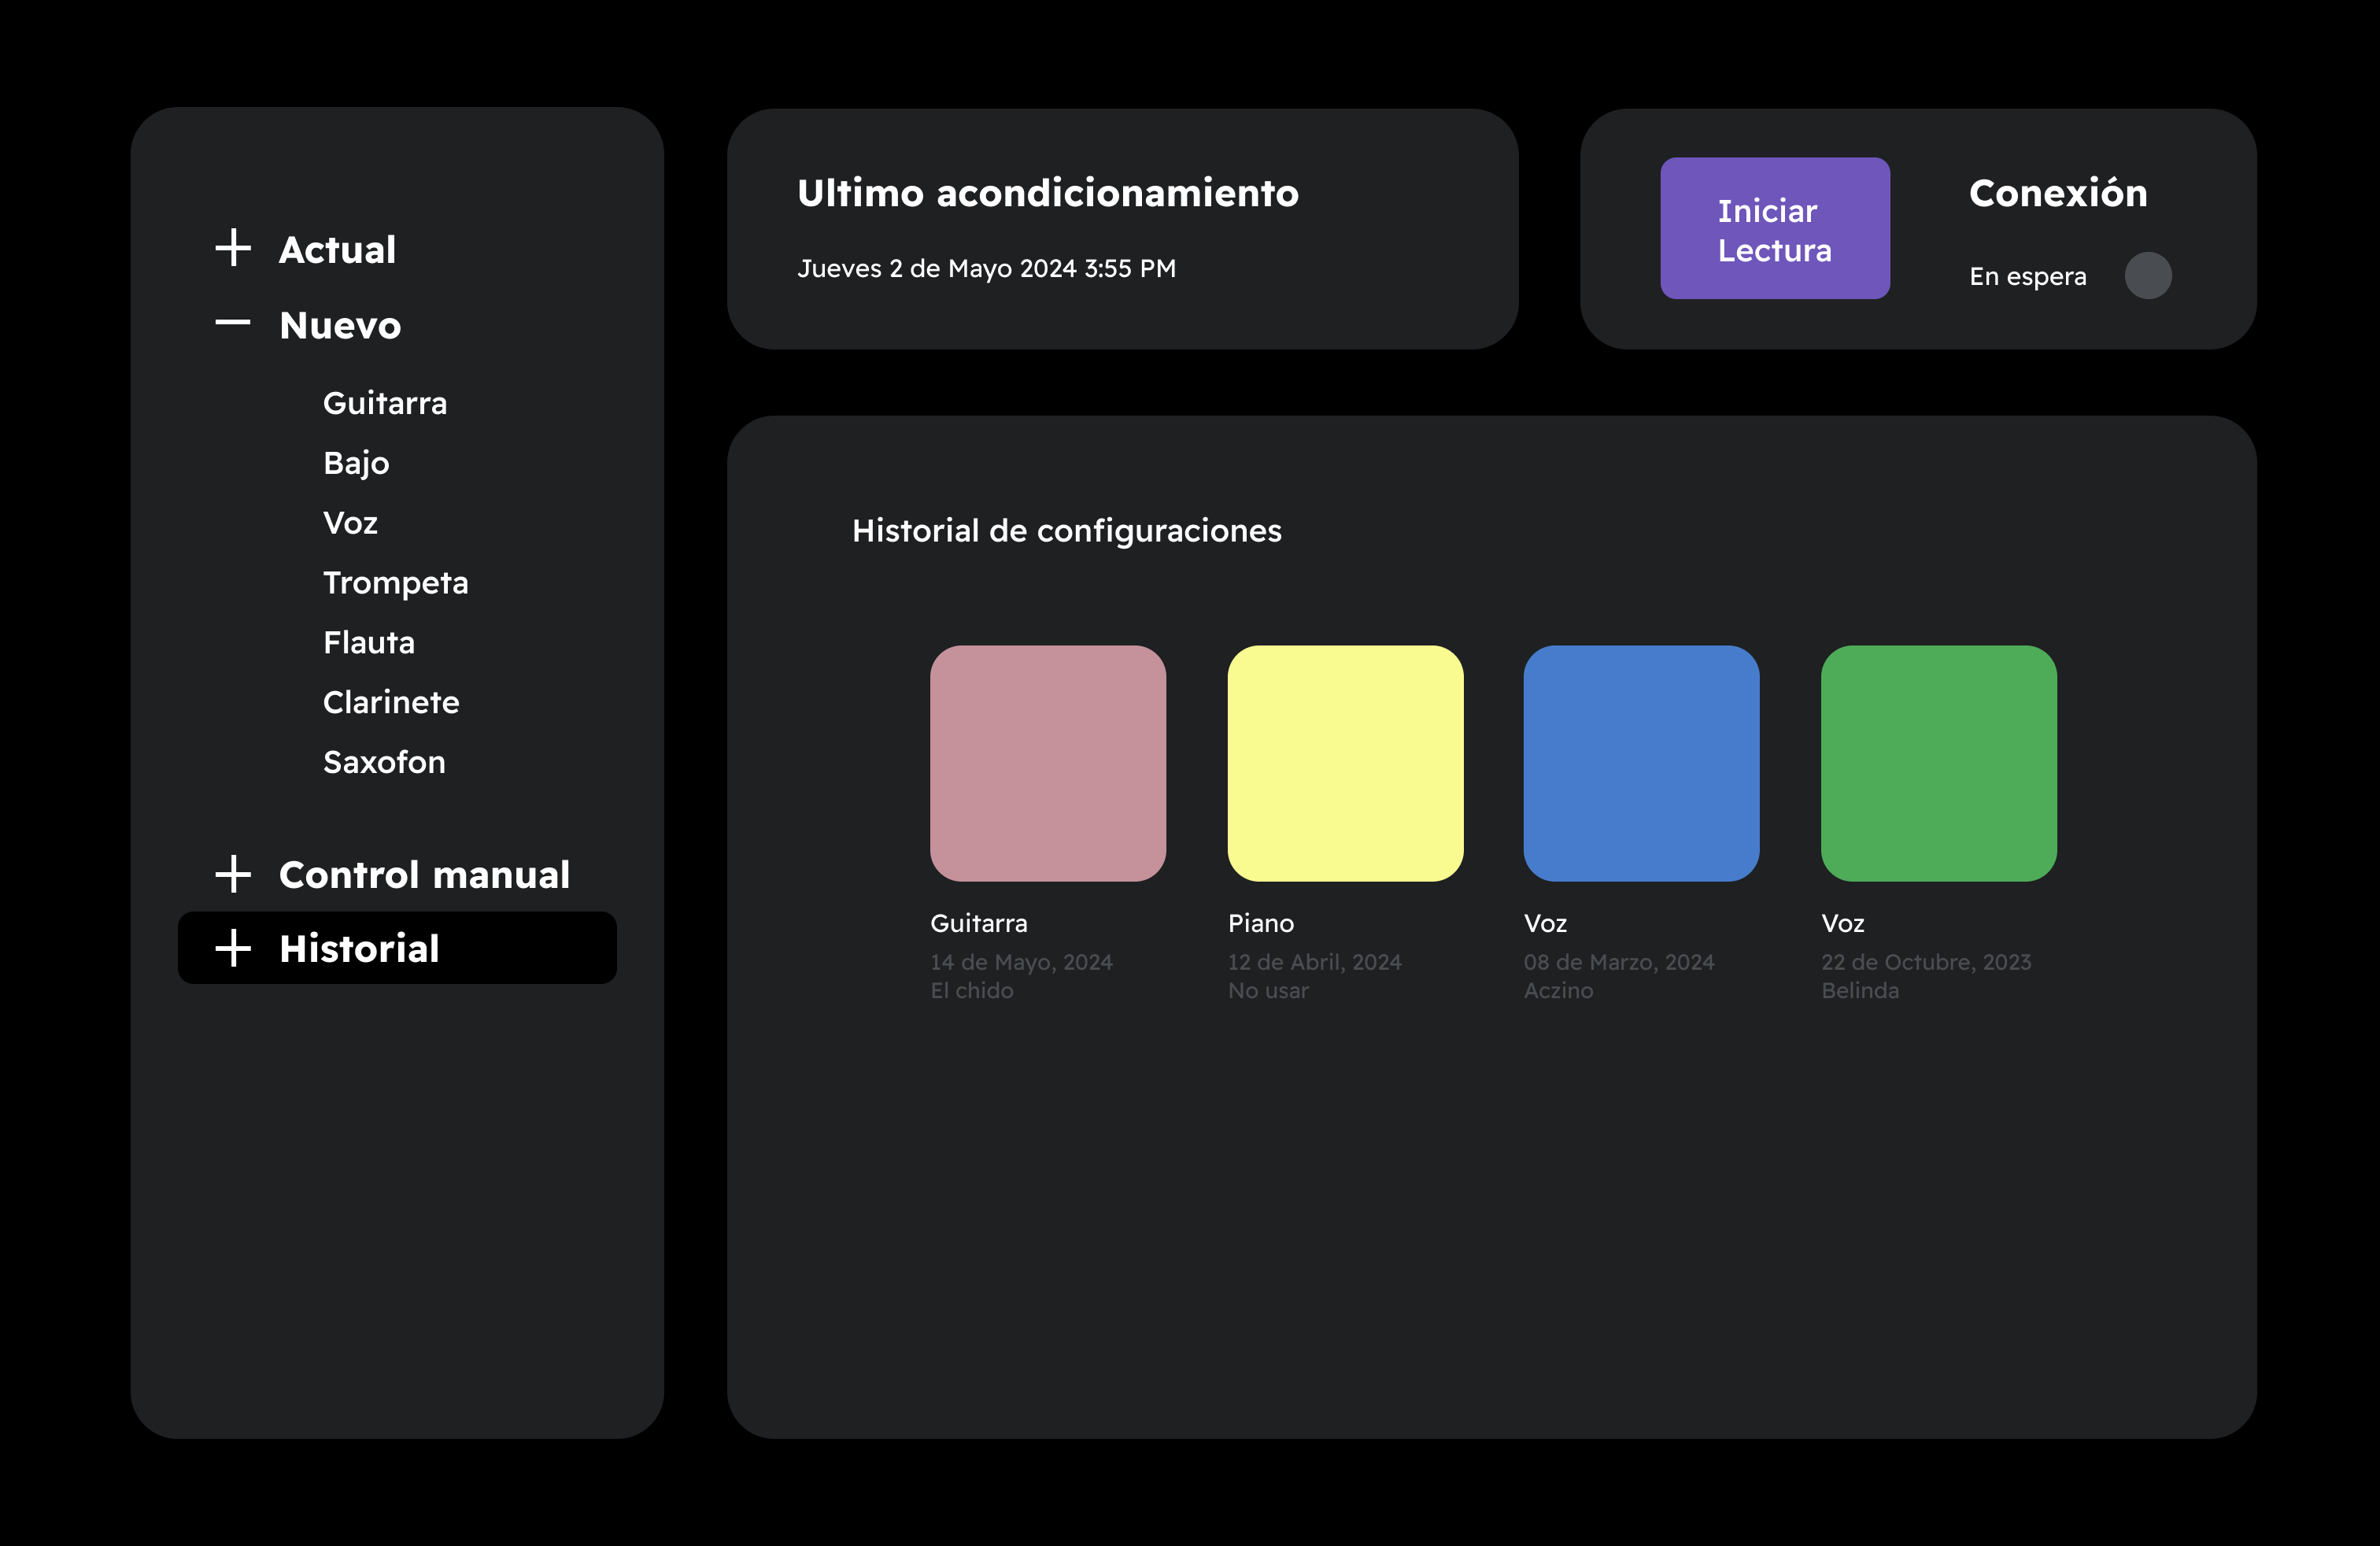
\includegraphics[width=\linewidth]{imagenes/Historial.png}
    \caption{\footnotesize Interfaz de usuario. Página del historial de configuraciones}
    \label{fig:DecayCurve}
\end{figure}
\FloatBarrier
